\documentclass{article}
\usepackage{amsmath, amssymb, cancel, mathtools, bm}
\usepackage[left=.5in, right=.5in, top=1in, bottom=1in]{geometry}
\usepackage[most]{tcolorbox}
\usepackage[skip=1em,indent=0pt]{parskip}
\setlength{\parindent}{0pt}
\newcommand{\statvec}[1]{\underset{\sim}{\bm{#1}}} % Vector symbol (tilde under vector)
\DeclareMathOperator{\EX}{\mathbb{E}} % Expected Value symbol
\newcommand{\indep}{\perp\!\!\!\!\perp} % Independence symbol
\newcommand{\real}{\mathbb{R}} % Simplified 'Reals' indicator
\newcommand{\pto}{\overset{P}{\to}}
\newcommand{\asto}{\overset{a.s.}{\to}}
\newcommand{\rthto}{\overset{L^r}{\to}}
\newcommand{\dto}{\overset{D}{\to}}
\newcommand{\ext}{\EX_{\theta}}
% Force all aggregate symbols to always put values above/below
\let\Oldint=\int
\let\Oldsum=\sum
\let\Oldprod=\prod
\let\Oldbigcup=\bigcup
\let\Oldbigcap=\bigcap
\let\Oldlim=\lim
\renewcommand{\int}{\Oldint\limits} 
\renewcommand{\sum}{\Oldsum\limits} 
\renewcommand{\prod}{\Oldprod\limits} 
\renewcommand{\bigcup}{\Oldbigcup\limits} 
\renewcommand{\bigcap}{\Oldbigcap\limits} 
\renewcommand{\lim}{\Oldlim\limits} 
\newcommand{\infint}{\int_{-\infty}^{\infty}}
\newcommand{\iiddist}{\overset{\mathrm{iid}}{\sim}}
\newcommand{\norm}[1]{\left\lVert#1\right\rVert}
\newcommand{\boldred}[1]{\textbf{\textcolor{red}{#1}}}


\begin{document}

\section{CB2 8.3}

$Y_i, ..., Y_m \sim Bern(\theta)$. Show that the LRT of $H_0: \theta \le \theta_0, H_1: \theta> \theta_0$ will reject if $\sum_{i=1}^m Y_i > b$

$L(Y|\theta) = \prod \theta^y(1-\theta)^{1-y} = \theta^{\sum y} (1-\theta)^{m-\sum y}$

LRT $= \frac{argmax L(\theta|Y)_{\Theta_0}}{argmax L(\theta|Y)_{\Theta}}$

The plot of the likelihood is basically a hill, and under the null, the argmax of the likelihood occurs at either $\theta_0$, or the MLE ($\bar{Y}$) (it is monotonic increasing up to that point). Over the full space, the argmax is at the MLE, $\bar{X} = \frac{\sum Y_i}{m}$ 

$\implies$ LRT $ = \frac{\theta_0^{\sum y} (1-\theta_0)^{m-\sum y}}{(\frac{\sum Y_i}{m})^{\sum y} (1-\frac{\sum Y_i}{m})^{m-\sum y}} = (\frac{m \theta_0}{\sum y})^{\sum y} (\frac{1 -\theta_0}{1-\sum y / m})^{m-\sum y}$, we will reject if that's less than $c$.

$ln(\lambda(x)) < ln(c) \implies \sum y (ln(m) + ln(\theta_0) - ln(\sum y)) + (m - \sum y)(ln(1-\theta_0) - ln(1 - \sum y /m)) < ln(c)$

Let $x = \sum y$:

$\frac{d}{dx} = ln(\theta_0) - ln(1-\theta_0) - ln(\frac{x}{m}) - 1 + ln(\frac{m-x}{m}) + 1 = ln(\frac{\theta_0 (\frac{m-y}{m})}{y/m(1-\theta_0)})$

In all cases, the fraction inside the log is less than 1, so the ln is negative, meaning this is a decreasing function, such that $\lambda(\sum y) < c \iff  \sum Y > b$

\section{CB2 8.6}

$X \iiddist Exp(\theta); Y \iiddist Exp(\mu)$

a) Find the LRT of $H_0: \theta = \mu, H_1: \theta \neq mu$

LRT $ = \frac{L(\hat{\theta}_{\Theta_0} | x, y)}{L(\hat{\theta}_{\Theta}|x,y)} = \frac{sup_{\theta}\frac{1}{\theta^n}e^{-\sum x / \theta}\frac{1}{\mu^m}e^{-\sum y/\mu}}{sup_{\theta, \mu}\frac{1}{\theta^n}e^{-\sum x / \theta}\frac{1}{\mu^m}e^{-\sum y/\mu}}$

In the numerator we are assuming that $\theta = \mu$

$\implies \frac{sup_{\theta}\frac{1}{\theta^{n+m}}e^{-(\sum x + \sum y)/ \theta}}{sup_{\theta, \mu}\frac{1}{\theta^n}e^{-\sum x / \theta}\frac{1}{\mu^n}e^{-\sum y/\mu}}$

The numerator: $\frac{d}{d\theta} = \frac{-(n+m)}{\theta^{n+m+1}}e^{-(\sum x + \sum y)/\theta} - \frac{\sum x + \sum y}{\theta^{n+m}}e^{-(\sum x + \sum y)/ \theta} = 0 \implies \hat{\theta}_0 = \frac{\sum x + \sum y}{n+m}$

In the denominator, the MLEs are just $\bar{x}$ and $\bar{y}$

$\implies \frac{L(\hat{\theta}_{\Theta_0} | x, y)}{L(\hat{\theta}_{\Theta}|x,y)} = \frac{(\frac{n + m}{\sum x + \sum y})^{n+m}e^{-\frac{n+m}{\sum x + \sum y}(\sum x + \sum y)}}{(\frac{n}{\sum x})^n e^{-\frac{n}{\sum x}\sum x}(\frac{m}{\sum y})^m e^{-\frac{m}{\sum y}\sum y}} = \frac{(n+m)^{n+m} (\sum x)^n (\sum y)^m}{n^n m^m (\sum x + \sum y)^{n+m}}$

Thus, LRT says we reject when $\frac{(n+m)^{n+m} (\sum x)^n (\sum y)^m}{n^n m^m (\sum x + \sum y)^{n+m}} \le c$

b) Show the test in part (a)can be based on statistic $T = \frac{\sum X_i}{\sum X_i + \sum Y_i}$

If $T = \frac{\sum X_i}{\sum X_i + \sum Y_i}$, then $1 - T = \frac{\sum Y_i}{\sum X_i + \sum Y_i}$

We can rewrite that test as: $\frac{(n+m)^{n+m}}{n^n m^m}(\frac{\sum x}{(\sum x + \sum y)})^n(\frac{\sum y}{(\sum x + \sum y)})^m = \frac{(n+m)^{n+m}}{n^n m^m} T^n (1-T)^m$

c) Find distribution of $T$ when $H_0$ is true

The sum of exponentials is a Gamma, so in this case $\sum x \sim Gamma(n, \theta); \sum y \sim Gamma(m, \mu)$. However, we are assuming the null hypothesis is true, so $\sum y \sim Gamma(m, \mu)$.

I had to look up what the distribution of $\frac{Gamma(n, \theta)}{Gamma(n, \theta) + Gamma(m, \theta)}$ is, turns out it's $Beta(n, m)$

Thus, the resulting distirbution of $T$ is $Beta(n,m)$

\section{CB2 8.7a}

a) 

$f(x|\theta, \lambda) = \frac{1}{\lambda} e^{-(x-\theta)/\lambda} I_{[\theta, \infty)}(x)$, both $\theta, \lambda$ unknown. $H_0: \theta \le 0, H_1: \theta > 0$. Find the LRT.

$L(\lambda, \theta | x) = \prod \frac{1}{\lambda}e^{-(x-\theta)/\lambda}I_{[\theta, \infty)}(x) = \frac{1}{\lambda^n}e^{-(\sum x - n\theta)/\lambda} I_{[\theta, \infty)}(X_{(1)})$

The marginal effect of $\theta$ is that as $\theta$ increases (irresepective of $\lambda$), the function is increasing (under condition that $\theta < x_{(1)}$). Thus, the $\hat{\theta} = x_{(1)}$

For $\lambda$: $\frac{d}{d\lambda} = \frac{-n}{\lambda}e^{-(\sum x - n\theta)/\lambda} - \frac{\sum x - n\theta}{\lambda^{n+1}}e^{-(\sum x - n\theta)/\lambda} = 0 \implies \frac{-n}{\lambda} = \frac{\sum x - n\theta}{\lambda^{n+1}} \implies n\lambda = \sum x - n\theta \implies \hat{\lambda} = \bar{x} - \hat{\theta} = \bar{x} - x_{(1)}$

Those values apply for the denominator. Now for the numerator, we are restricted to $\theta \le 0$. Thus, if $x_{(1)} > 0$, that is not allowed so the MLE would be $0$. So we have $\hat{\theta}_R = \begin{cases} x_{(1)}, & x_{(1)} \le 0 \\ 0, & x_{(1)} > 0 \end{cases}$

Looking at our above value for $\lambda$, we plug in $\hat{\theta}_R = 0$ and get $\hat{\lambda}_R = \bar{x}$

Now we do the ratio; $\lambda(x) = \frac{L(\hat{\theta}_R, \hat{\lambda}_R|x)}{L(\hat{\theta}, \hat{\lambda}|x)} = \frac{\frac{1}{\bar{x}^n}e^{-(\sum x - n x_{(1)})/\bar{x}}}{\frac{1}{(\bar{x} - x_{(1)})^n} e^{-(\sum x - n x_{(1)})/(\bar{x} - x_{(1)})}} = (\frac{\bar{x} - x_{(1)}}{\bar{x}})^n = (1 - \frac{x_{(1)}}{\bar{x}})^n$

Thus, LRT says we reject when $\lambda(x) \le c$, which is equivalent to rejecting when $\frac{x_{(1)}}{\bar{x}} \le a$ for some a. 

\section{CB2 8.8a or CB2 8.8b}

a) $X \sim N(\theta, \alpha \theta), \theta$ unknown. Find the LRT of $H_0: \alpha = 1, H_1: \alpha \neq 1$

$L(\theta, a |x) = (2\pi a\theta)^{-n/2}e^{-\frac{1}{2a\theta}\sum (x_i - \theta)^2}$

$\implies ln(L) = -\frac{1}{2}\sum [ln(2\pi a\theta) + \frac{1}{a\theta}(x_i-\theta)^2]$

$\implies \frac{\partial}{\partial a} = -\frac{1}{2}\sum[\frac{1}{a} - \frac{1}{a^2\theta}(x_i - \theta)^2] = -\frac{n}{2a} + \frac{1}{2a^2 \theta}\sum(x_i - \theta)^2 = 0 \implies \frac{n}{2a} = \frac{1}{2a^2 \theta}\sum(x_i - \theta)^2 \implies a = \frac{1}{n\theta}\sum(x_i - \theta)^2$

$\implies \frac{\partial}{\partial \theta} = -\frac{n}{2\theta} + \sum[\frac{1}{2a\theta^2}(x_i-\theta)^2 + \frac{2(x_i - \theta)}{2a\theta}] = 0 \implies \frac{n}{2\theta} = \frac{1}{2a\theta^2}\sum(x_i - \theta)^2 + \frac{n\bar{x} - n\theta}{a\theta}$

Plug the first equation into the second: $\frac{n}{2\theta} = \frac{n\theta\sum(x_i - \theta)^2}{2\theta^2\sum(x_i - \theta)^2} + \frac{(n\bar{x} - n\theta)n\theta}{\theta\sum(x_i - \theta)^2} = \frac{n}{2\theta} + \frac{(n\bar{x} - n\theta)n}{\sum(x_i - \theta)^2} \implies 0 = \frac{(n\bar{x} - n\theta)n}{\sum(x_i - \theta)^2} \implies \hat{\theta} = \bar{x}$

Plug that back into the first: $a = \frac{1}{n\bar{x}}\sum(x_i - \bar{x})^2 = \frac{\sigma^2}{\bar{x}}$

Those are the unrestricted MLEs. For the supremums under the null, we let a=1. Going bacl to our previous equations: $a = 1 = \frac{n}{\theta}\sum(x_i - \theta)^2 \implies n\theta = \sum (x_i - \bar{x})^2 + n(\bar{x} - \theta)^2 \implies \theta = \sigma^2 + \bar{x}^2 - 2\bar{x}\theta + \theta^2 \implies \hat{\theta}_R = \frac{-1 + \sqrt{1 + 4(\hat{\sigma} + \bar{x}^2)}}{2}$

This gives the LRT: $\lambda(x) = \frac{L(\hat{\theta}_R|x)}{L(\hat{a},\hat{\theta}|x)} = \frac{(2\pi \hat{\theta}_R)^{-n/2}e^{-\frac{1}{2\hat{\theta}_R}\sum (x_i - \theta)^2}}{(2\pi \hat{a}\hat{\theta})^{-n/2}e^{-\frac{1}{2\hat{a}\hat{\theta}}\sum (x_i - \theta)^2}} = \frac{(2\pi \hat{\theta}_R)^{-n/2}e^{-\frac{1}{2\hat{\theta}_R}\sum (x_i - \theta)^2}}{(2\pi \hat{\sigma}^2)^{-n/2}e^{-\frac{1}{2\hat{\sigma}^2}\sum (x_i - \theta)^2}} = \underline{(\frac{\hat{\sigma}^2}{\hat{\theta}_R})^{n/2}e^{(n/2) - \sum\frac{(x_i - \hat{\theta}_R)^2}{2\hat{\theta}_R}}}$ with $\hat{\theta}_R$ as described above. 

\section{}

$X_i \iiddist Pois(\theta), \theta > 0$

a) 

Show that LRT for $H_0: \theta = \theta_0, H_1: \theta \neq \theta_0$ can be written as $\phi(x) = \begin{cases} 1, & \sum X_i \notin [k_1,k_2] \\ 0, & \sum X_i \in [k_1,k_2] \end{cases}, k_1, k_2 > 0$

$L(\theta|x) = \prod \frac{\theta^x e^{-\theta}}{x!} = \frac{\theta^{\sum x} e^{-n\theta}}{\prod x!}$

The unrestricted MLE for $\theta = \hat{\theta} = \bar{X}$

Under the restrcition that $\theta = \theta_0$, then $\hat{\theta}_R = \theta_0$

LRT $= \frac{L(\hat{\theta}_R|x)}{L(\hat{\theta}|x)} = \frac{\theta_0^{\sum x} e^{-n\theta_0}}{\bar{x}^{\sum{x}}e^{-n\bar{x}}} = \left( \frac{\theta_0}{\bar{x}}\right)^{\sum x}e^{-n(\theta_0 + \bar{x})}$

The LRT says we will reject when $\left( \frac{\theta_0}{\bar{x}}\right)^{\sum x}e^{-n(\theta_0 + \bar{x})} \ge a$ or $\le b$. In this case, this is just an increasing function of $\sum x$, meaning this is equivalent to rejecting when $\sum x \le k_1$ or $\sum x \ge k_2$.

This can be written as: $\phi(x) = \begin{cases} 1, & \sum X_i \notin [k_1,k_2] \\ 0, & \sum X_i \in [k_1,k_2] \end{cases}$

b) 

$n=5, \alpha = 0.05, \theta_0 = 2$, find $k_1, k_2$ such that LRT has as close as possible, but not exceeding $\alpha = 0.05$

The sum of Poissons is a Poisson with the sum of the variables, so $\sum x \sim Pois(\theta_0*n) = Pois(10)$

We basically need to solve $P(k1 \le \sum x \le k_2) = 1-\alpha \implies P(\sum x \le k_2) - P(\sum x \le k_1) = 1- \alpha \implies P(\sum x \le k_2) - P(\sum x \le k_1) - 1 + \alpha = 0$. 

We can then use root finding to get that value. I used the following r code: 
\begin{verbatim}
func <- function(params) {
  k1 <- params[[1]]
  k2 <- params[[2]]
  ppois(k1, 10) - ppois(k2, 10) - 1 + .05
}

optim(par = c(1, 20), func)
\end{verbatim}

and got a value of: $k_1 = -31.5, k_2 = 47.125$

\section{}

$X = (X_1, X_2, X_3)$ is trinomial: $p = (p_1, p_2, p_3)$ wiht PMF $f(x|p) = \prod_{j=1}^3 p_j^{x_j}; \sum_{j=1}^3 x_j = m; p_j > 0, \sum p_j = 1$.

Let $m=1$, and for $\theta \in (-1, 1): p_1 = \frac{(1-\theta)^2}{4}; p_2 = \frac{(1-\theta^2)}{2}, p_3 = \frac{(1+\theta)^2}{4}$

a)

Let $Y_j = \sum_{i=1}^n X_{ij}$. Show that MLE $\hat{\theta} = \frac{Y_3 - Y_1}{n}$

$f(x|\theta) = \left( \frac{(1-\theta)^2}{4} \right)^{x_1}\left( \frac{1-\theta^2}{2}\right)^{x_2}\left( \frac{(1+\theta)^2}{4}\right)^{x_3} = \frac{(1-\theta)^{2x_1}(1-\theta^2)^{x_2}(1+\theta)^{2x_3}}{2^{2x_1}2^{x_2}2^{2x_3}}$

$L(\theta|x) = \prod_{i=1}^n f(x|\theta) = \frac{(1-\theta)^{2\sum x_{1,i}}(1-\theta^2)^{\sum x_{2,i}}(1+\theta)^{2 \sum x_{3,1}}}{2^{2 \sum x_{1,1}}2^{\sum x_{2,1}}2^{2 \sum x_{3,i}}} = \frac{(1-\theta)^{2Y_1}(1-\theta^2)^{Y_2}(1+\theta)^{2 Y_3}}{2^{2 Y_1}2^{Y_2}2^{2 Y_3}}$

$ln(L(\theta|x)) = 2Y_1 ln(1-\theta) + Y_2 ln(1-\theta^2) + 2Y_3 ln(1+\theta) - (2Y_1 + Y_2 + 2Y_3)ln(2)$

$\frac{d}{d\theta} ln(L(\theta|x)) = -\frac{2Y_1}{1-\theta} - \frac{2Y_2\theta}{1-\theta^2} + \frac{2Y_3}{1+\theta} = 0 = -\frac{Y_1}{1-\theta} - \frac{Y_2\theta}{1-\theta^2} + \frac{Y_3}{1+\theta} \implies -\frac{Y_1(1-\theta^2)(1+\theta)-Y_2 \theta(1-\theta)(1+\theta) + Y_3(1-\theta)(1-\theta^2)}{STUFF} = 0$

$\implies -Y_1(1 - \theta^2 + \theta - \theta^3)- Y_2(\theta - \theta^3) + Y_3(1 - \theta - \theta^2 + \theta^3) = 0$

$\implies (Y_3 - Y_1) - \theta(Y_1 + Y_2 + Y_3) + \theta^2(Y_1 - Y_3) + \theta^3(Y_1 + Y_2 + Y_3) = 0$

Since $\sum_{j=1}^3 = m = 1 \implies Y_1 + Y_2 + Y_3 = n$

$\implies (Y_3 - Y_1) - n\theta - \theta^2(Y_3 - Y_1) + n\theta^3 = (Y_3 - Y_1)(1-\theta^2) + n\theta(\theta^2-1) = (Y_1 - Y_3)(\theta^2 - 1) + n\theta(\theta^2 - 1) = 0$

$\implies (Y_1 - Y_3) + n\theta = 0 \implies \hat{\theta} = \frac{Y_3 - Y_1}{n}$

b)

Find, as simple form as possible, asymptotic size $\alpha$ rejection regions for Generalized LRT for $H_0:\theta = 0, H_1:\theta \neq 1$

We just found the unrestricted MLE. To find the restricted MLE, we are saying that $\hat{\theta}_R = 0$, so we will just plug that in anywhere we have 0. 

LRT $ = \frac{L(\hat{\theta}_R|x)}{L(\hat{\theta}|x)} = \frac{\frac{(1-0)^{2Y_1}(1-0^2)^{Y_2}(1+0)^{2Y_3}}{2^{2Y_1 + Y_2 + 2Y_3}}}{\frac{(1-\hat{\theta})^{2Y_1}(1-\hat{\theta}^2)^{Y_2}(1+\hat{\theta})^{2Y_3}}{{2^{2Y_1 + Y_2 + 2Y_3}}}} = \frac{1}{(1-\hat{\theta})^{2Y_1}(1-\hat{\theta}^2)^{Y_2}(1+\hat{\theta})^{2Y_3}}$

Thus, we reject anytime $ \frac{1}{(1-\hat{\theta})^{2Y_1}(1-\hat{\theta}^2)^{Y_2}(1+\hat{\theta})^{2Y_3}} \notin (c_1,c_2)$.

We can then use the Wilks' Theorem: $-2ln(\lambda) \dto \chi^2_1$

So our region is rejecting when $\lambda \notin (k_1,k_2)$ where $k_1$ fulfills: $P(\chi^2_1 \le -2ln(k_1)) = \alpha_1$ and $k_2$ fulfills: $P(\chi^2_1 \ge -2ln(k_2)) = \alpha_2$, and $\alpha_1 + \alpha_2 = \alpha$

c)

\begin{verbatim}
n <- 100
theta <- seq(-9, 9, by = 1)/10
alpha <- .05
# Assuming equal sided
lower <- qchisq(alpha/2, 1)
upper <- qchisq(1-alpha/2,1)
n_sim <- 500

power <- numeric(length(theta))
for (i in 1:length(theta)) {
  p1 <- (1-theta[[i]])^2/4
  p2 <- (1-theta[[i]]^2)/2
  p3 <- (1+theta[[i]])^2/4

  val <- numeric(length(n_sim))
  for (j in 1:n_sim) {
    dt <- rmultinom(n, size = 3, prob = c(p1,p2,p3))
    Y1 <- sum(dt[1,])
    Y2 <- sum(dt[2,])
    Y3 <- sum(dt[3,])
    theta_hat <- (Y3 - Y1)/n
    val[[j]] <- (1-theta_hat)^(2*Y1)*(1-theta_hat^2)^(Y2)*(1+theta_hat)^(2*Y3)
  }

  power[[i]] <- mean(val > upper | val < lower)
}

plot(theta, power)
\end{verbatim}

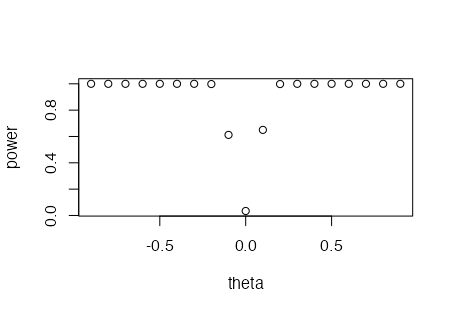
\includegraphics{power.png}

We can see that as $\theta$ moves away from the Null hypothesis, the Power increases and approaches 1. 

\end{document}